\documentclass{beamer}

\usepackage{graphicx}
\usepackage{tikz}
\usetheme{Frankfurt}

\title{The Scrum Method}
\author{Jimmy Mousel, Colin Holler, Dimitri Klockenbring, Jérémie Muzet, Céline Van Landeghem}
\date{}



\begin{document}



\frame{\titlepage}



\section{Summary}

\begin{frame}
    \frametitle{Table of content}
    \tableofcontents
\end{frame}



\section{What is Scrum?}

\begin{frame}
    \frametitle{What is Scrum ?}
    \begin{block}
        \onslide<1-> Scrum is one of the most used agile method.
        \begin{center}
            \onslide<1-> Empiricism \onslide<1-> - Participation \onslide<1-> - Self-organization
        \end{center}
    \end{block}
    \pause
    \begin{block}
        \onslide<2-> Scrum can be broken down into
        \begin{center}
            \onslide<2-> Roles \onslide<2-> - Events \onslide<2-> - Artifacts
        \end{center}
    \end{block}
\end{frame}

\begin{frame}
    \frametitle{What is Scrum ?}
    
    \framesubtitle{Roles}
    \begin{columns}
        \colon{.5\textwidh}
        \begin{block}{Roles}
            \begin{itemize}
                \item Product Owner
                
                \item Scrum Master
                
                \item Development Team
            \end{itemize}
        \end{block}
    
    
        \colon{.5\textwidh}
        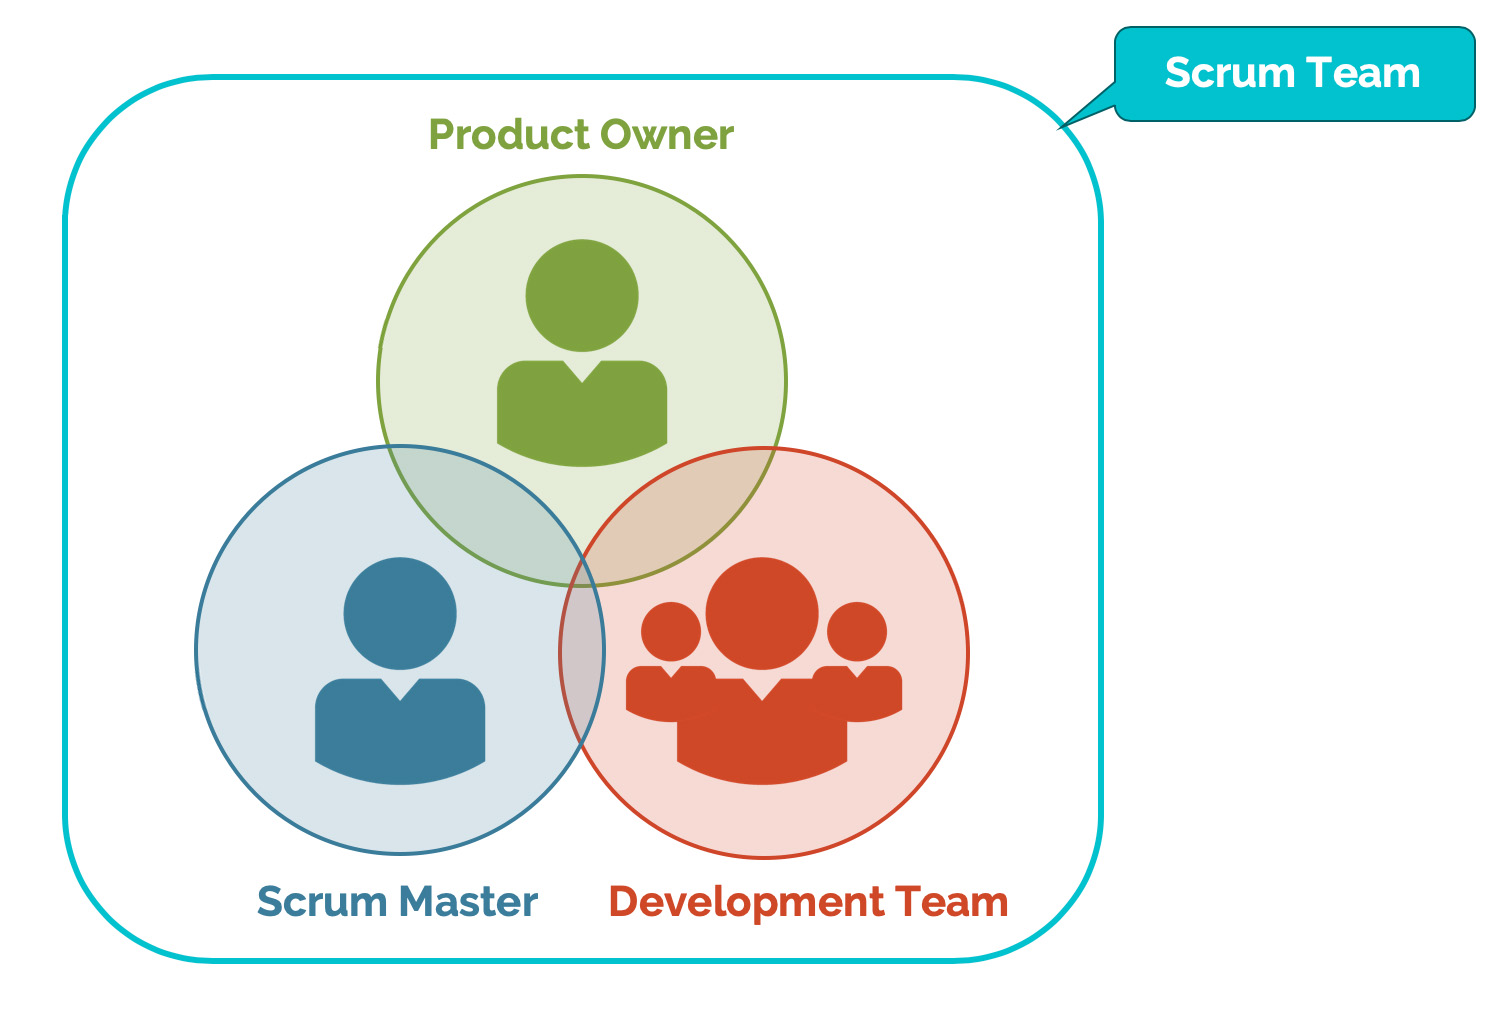
\includegraphics[width=1\textheight]{Images/roles.jpg}
    \end{columns}
    

    
\end{frame}



\section{The Scrum Workflow}

\begin{frame}
    \frametitle{Second slide}
    \begin{center}
	% à ordonner correctement :%
	% l'origine est en bas à gauche %
	% juste à gauche de "rectangle" on met les coordonnées du coin inf gauche
	% juste à droite de "rectangle" on met les coordonnées du point sup droit
        % Dans les chevrons après "draw" on indique à quel moment ça s'affiche
	\begin{tikzpicture}
            \node[anchor=south west,inner sep=0] at (0,0) {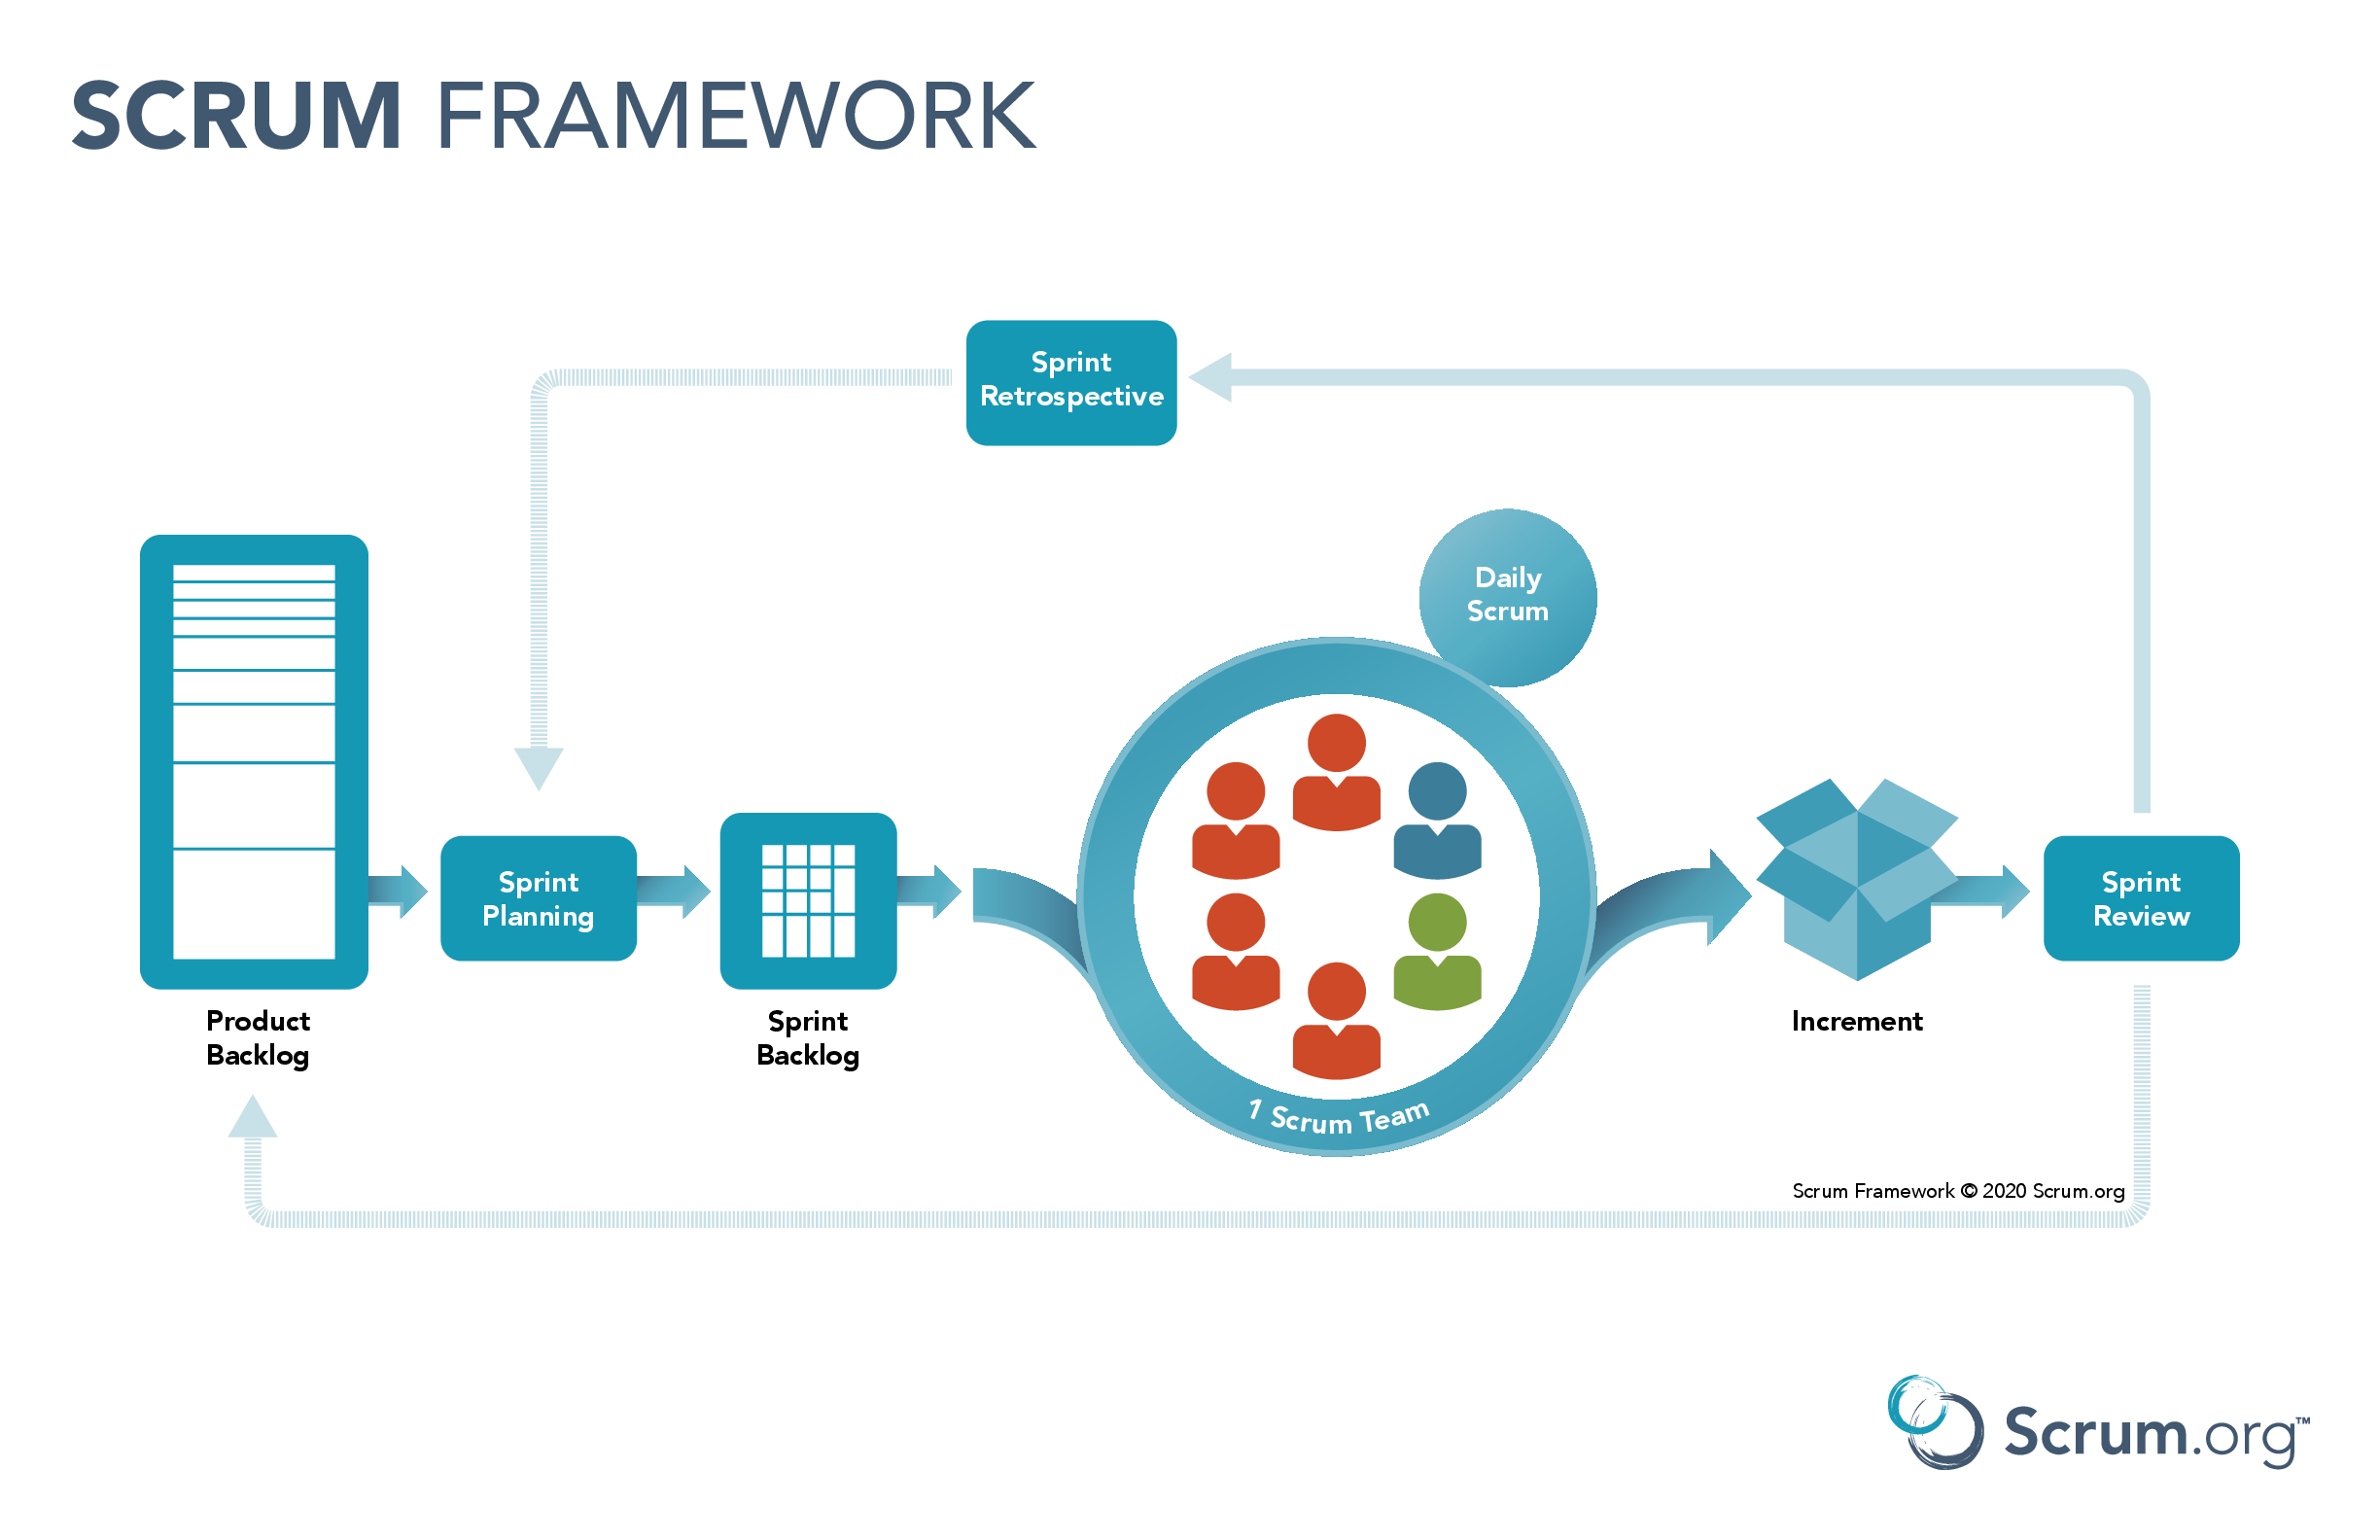
\includegraphics[width=1\textheight]{Images/Scrumorg-Scrum-Framework}};
            \draw<1>[red,ultra thick,rounded corners] (0.4,1.6) rectangle (1.5,4);
            \draw<2>[red,ultra thick,rounded corners] (1.5,2) rectangle (2.5, 2.8);

	    \draw<3>[red,ultra thick,rounded corners] (2.6,1.6) rectangle (3.5, 2.9);
	    \draw<4>[red,ultra thick,rounded corners] (5.2,3.1) rectangle (6.1, 4);
	    \draw<5>[red,ultra thick,rounded corners] (6.5,1.7) rectangle (7.5, 3);
	    \draw<6>[red,ultra thick,rounded corners] (7.5,2) rectangle (8.5, 2.8);
	    \draw<7>[red,ultra thick,rounded corners] (3.5,4) rectangle (4.5, 4.7);

	    \draw<8>[red,ultra thick,rounded corners] (1.5,2) rectangle (2.5, 2.8);
	    \draw<9>[red,ultra thick,rounded corners] (2.6,1.6) rectangle (3.5, 2.9);
	    \draw<10>[red,ultra thick,rounded corners] (5.2,3.1) rectangle (6.1, 4);
	    \draw<11>[red,ultra thick,rounded corners] (6.5,1.7) rectangle (7.5, 3);
	    \draw<12>[red,ultra thick,rounded corners] (7.5,2) rectangle (8.5, 2.8);
	    \draw<13>[red,ultra thick,rounded corners] (3.5,4) rectangle (4.5, 4.7);

	    \draw<14>[red,ultra thick,rounded corners] (1.5,2) rectangle (2.5, 2.8);
	    \draw<15>[red,ultra thick,rounded corners] (2.6,1.6) rectangle (3.5, 2.9);
	    \draw<16>[red,ultra thick,rounded corners] (5.2,3.1) rectangle (6.1, 4);
	    \draw<17>[red,ultra thick,rounded corners] (6.5,1.7) rectangle (7.5, 3);
	    \draw<18>[red,ultra thick,rounded corners] (7.5,2) rectangle (8.5, 2.8);
	    \draw<19>[red,ultra thick,rounded corners] (3.5,4) rectangle (4.5, 4.7);
	    
        \end{tikzpicture}
    \end{center}
    
\end{frame}



\section{Advantages \& Disadvantages}

\begin{frame}
    \frametitle{Advantages and Disadvantages}
    
    \begin{columns}
    
    \column{0.5\textwidth}
    Advantages
    \begin{itemize} 
    \item<2-> Sprints : quick adaption, flexibility
    \item<3-> Meetings : daily update
    \item<4-> More responsibility, higher productivity
    \item<5-> Increase in customer satisfaction
    \end{itemize}
    
    \column{0.5\textwidth}
    Disadvantages
    \begin{itemize}
    \item<6-> Effectiveness depends on the team
    \item<7-> Members not experienced : Project tends to fail
    \item<8-> Daily meetings are excessive
    \item<9-> Method can be difficult to apply
    \end{itemize}
    \end{columns}
\end{frame}



\section{Scrum and GitHub}

\begin{frame}
    \frametitle{SCRUM and GitHub}
    \begin{itemize}
    \color{gray}
    \item[•] Sprints
    \item[•] \textcolor{black}{Issues}
    \item[•] GitScrum
    \end{itemize}
\end{frame}



\section{Bibliography}

\begin{frame}
    \frametitle{Bibliography}
	\begin{thebibliography}{10}

	\bibitem{ScrumOnGithub}
	\textit{Software Development Practices with GitHub} \\
	\texttt{https://www.scrumassembly.org/Library/ScrumMastery/ISM/\\
	International+Scrum\%E2\%84\%A2/Software+Development+Practices+with+GitHub}

	\bibitem{agile}
	\textit{How To Use GitHub for Agile Project Management} \\
	\texttt{https://blog.zenhub.com/how-to-use-github-agile-project-management/}
	\end{thebibliography}
\end{frame}

\end{document}